% Based on Template from IIS, ETHz
%%%%%%%%%%%%%%%%%%%%%%%%%%%%%%%%%%%%%%%%%%%%%%%%%%%%%%%%%%%%%%%%%%%%%%%
%%%%%%%%%%%%%%%%%%%%%%%%%%%%%%%%%%%%%%%%%%%%%%%%%%%%%%%%%%%%%%%%%%%%%%%
%%%%%                                                                 %
%%%%%     <file_name>.tex                                             %
%%%%%                                                                 %
%%%%% Author:      <author>                                           %
%%%%% Created:     <date>                                             %
%%%%% Description: <description>                                      %
%%%%%                                                                 %
%%%%%%%%%%%%%%%%%%%%%%%%%%%%%%%%%%%%%%%%%%%%%%%%%%%%%%%%%%%%%%%%%%%%%%%
%%%%%%%%%%%%%%%%%%%%%%%%%%%%%%%%%%%%%%%%%%%%%%%%%%%%%%%%%%%%%%%%%%%%%%%

\chapter{Results}\label{section:results}
% First describe your measurement setup and settings (so it could be reproduced) and afterwards describe the results you got from your experiments. Putting results in perspective and interpretation do not belong in this chapter (put that into the discussion)

Although cycle counting and timing are possible on external hardware, the most accurate results can be obtained by simulating fixed dive profiles to compare the different algorithms. 
A fixed-voltage DC Power Supply that has been set to output $\SI{3.7}{\volt}$ is used to provide power to the \gls{pcb}.
The software is programmed onto the MCU using the 6-pin JTAG connector \emph{J1} via a STLink V3SET.

The software can be configured using the Rust Build System \lstinline{cargo}'s \lstinline{feature} flags, which can be used for conditional compilation. 
To simplify interaction with different setups, a \lstinline{Justfile} is provided for the \lstinline{just} command runner. 
The standard dive computer application can be flashed using \lstinline{just embed}, while live simulation and result extraction can be obtained by running \lstinline{just embed-live-sim-log-DEPTH(-FEATURE)}, where \lstinline{DEPTH} can be one of \lstinline{20m}, \lstinline{50m} and \lstinline{90m} and \lstinline{FEATURE} is optional, may be \lstinline{exp} or \lstinline{fixed-rate}.

The following figures are generated from the \texttt{csv} files that are output from the \texttt{extract\_\-bench\_\-tables.py} script in the project repository.
No preprocessing steps are performed except to clean up invalid characters in the exported log.
The figure generation scripts are available in the thesis repository and are also run automatically once a commit is pushed to GitHub via GitHub Actions, namely \texttt{generate\_\-decision\_\-summary.py}, \texttt{generate\_\-timing\_\-summary.py} and \texttt{generate\_\-dive\_\-profile\_\-graphics.py}.

The fixed rate simulations serve as the baseline for comparison, while the \lstinline{exp} ones enable the exponential and the recipes without \lstinline{FEATURE} run the linear-exponential algorithm.

\begin{figure}[htbp]
\centering
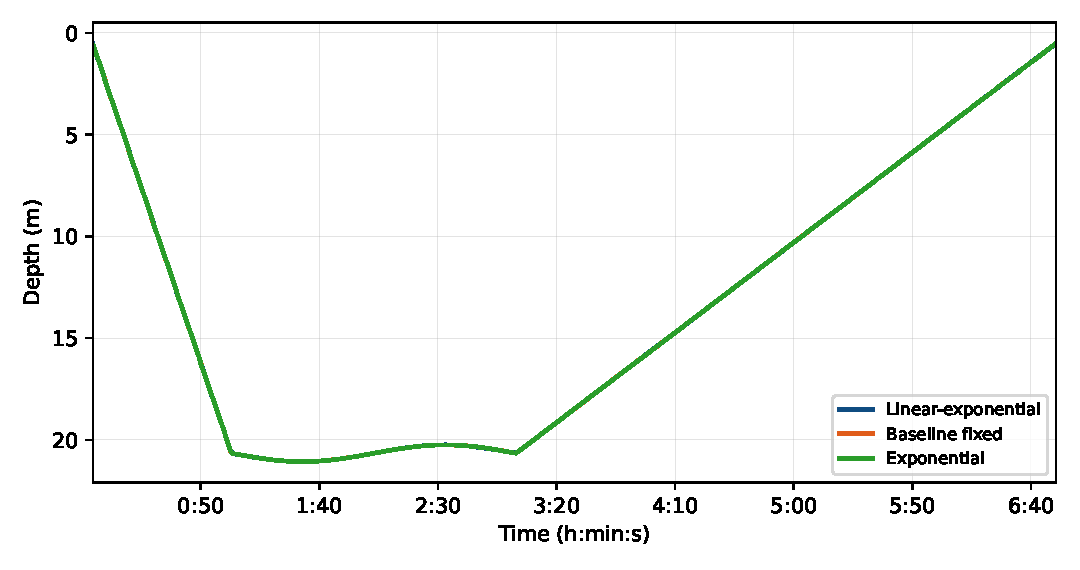
\includegraphics[width=0.9\textwidth]{figures/results/profile_20m.pdf}
\caption{Simulated Depth of 20m profile}
\label{fig:profile_20m}
\end{figure}

\begin{figure}[htbp]
\centering
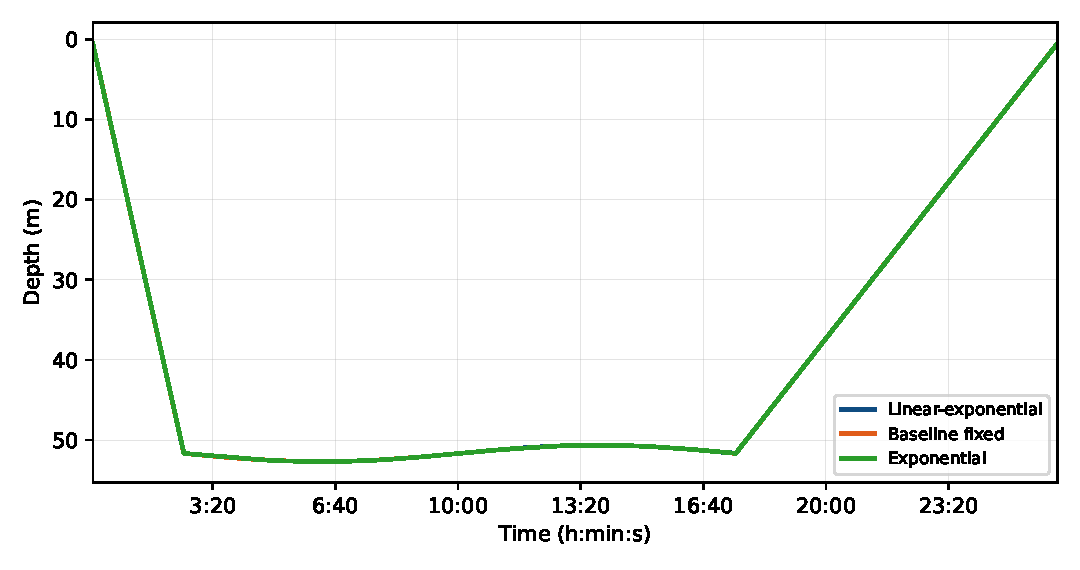
\includegraphics[width=0.9\textwidth]{figures/results/profile_50m.pdf}
\caption{Simulated Depth of 50m profile using the lin-exp decompression algorithm}
\label{fig:profile_50m}
\end{figure}

\begin{figure}[htbp]
\centering
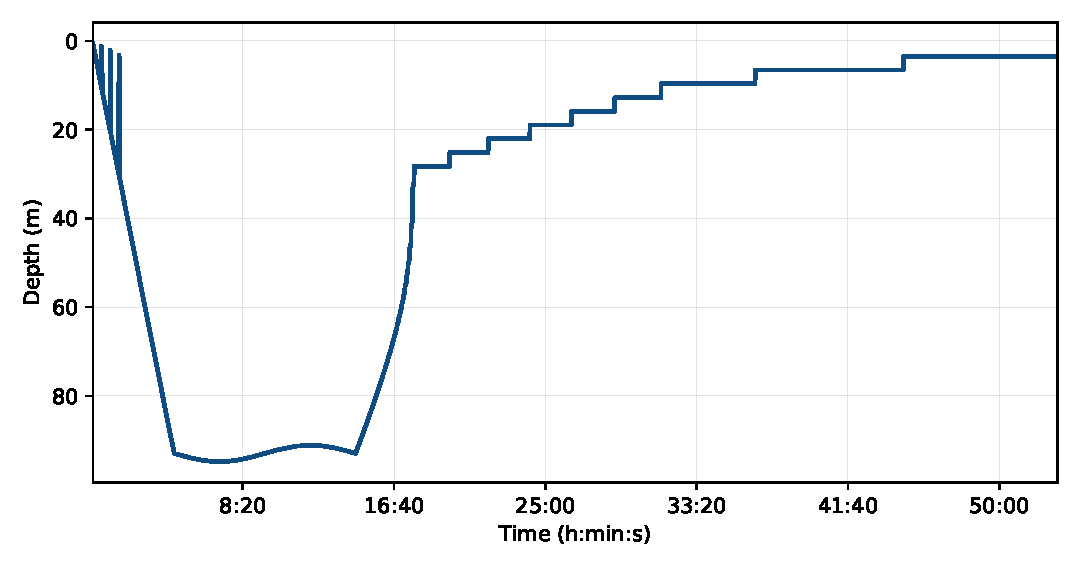
\includegraphics[width=0.9\textwidth]{figures/results/profile_90m.pdf}
\caption{Simulated Depth of 90m profile using the lin-exp decompression algorithm}
\label{fig:profile_90m}
\end{figure}

\section{\gls{o2tox} Algorithm results}
The implemented oxygen toxicity algorithm is only differential, runs on just one new measurement, and thus is comparatively cheap. 
The cycle count per execution of the fixed-rate algorithm, $235 \pm 2$, is only $10\%$ smaller than the execution of \gls{o2tox} itself, which is $266 \pm 2$.
This difference will become larger if more samples are used per-iteration.
The variable rate algorithms are on average $12.16\times$ more expensive, $1858 \pm 32$.

\begin{table}[htbp]
\centering
\small
\renewcommand{\arraystretch}{1.15}
\resizebox{\textwidth}{!}{%
\begin{tabular}{llrrrrrrrrrr}
\toprule
Configuration & Profile & Samples & Avg cycles & Avg [\si{\micro\second}] & Median cycles & Median [\si{\micro\second}] & Min cycles & Min [\si{\micro\second}] & Max cycles & Max [\si{\micro\second}] & Total cycles & Total [\si{\milli\second}] \\
\midrule
Baseline fixed & 20m & 8 & 265 & 16.6 & 265 & 16.6 & 265 & 16.6 & 265 & 16.6 & 2120 & 0.1 \\
Baseline fixed & 50m & 42 & 266 & 16.6 & 266 & 16.6 & 266 & 16.6 & 266 & 16.6 & 11172 & 0.7 \\
Baseline fixed & 90m & 87 & 266 & 16.6 & 266 & 16.6 & 266 & 16.6 & 266 & 16.6 & 23142 & 1.4 \\
Exponential & 20m & 1 & 265 & 16.6 & 265 & 16.6 & 265 & 16.6 & 265 & 16.6 & 265 & 0.0 \\
Exponential & 50m & 27 & 265 & 16.6 & 265 & 16.6 & 265 & 16.6 & 265 & 16.6 & 7155 & 0.4 \\
Exponential & 90m & 26 & 266 & 16.6 & 266 & 16.6 & 266 & 16.6 & 266 & 16.6 & 6916 & 0.4 \\
Linear-exponential & 20m & 1 & 267 & 16.7 & 267 & 16.7 & 267 & 16.7 & 267 & 16.7 & 267 & 0.0 \\
Linear-exponential & 50m & 34 & 266 & 16.6 & 266 & 16.6 & 266 & 16.6 & 266 & 16.6 & 9044 & 0.6 \\
Linear-exponential & 90m & 27 & 265 & 16.6 & 265 & 16.6 & 265 & 16.6 & 265 & 16.6 & 7155 & 0.4 \\
\bottomrule
\end{tabular}%
}
\caption{O\textsubscript{2} toxicity computation time across profiles and configurations}
\label{tab:timing_o2tox}
\end{table}

\begin{table}[htbp]
\centering
\small
\renewcommand{\arraystretch}{1.15}
\resizebox{\textwidth}{!}{%
\begin{tabular}{llrrrrrrrrr}
\toprule
Configuration & Profile & Samples & Avg cycles & Avg [\si{\micro\second}] & Min cycles & Min [\si{\micro\second}] & Max cycles & Max [\si{\micro\second}] & Total cycles & Total [\si{\milli\second}] \\
\midrule
Baseline fixed & 20m & 1833 & 237 & 14.8 & 237 & 14.8 & 237 & 14.8 & 434421 & 27.2 \\
Baseline fixed & 50m & 7778 & 234 & 14.6 & 234 & 14.6 & 234 & 14.6 & 1820052 & 113.8 \\
Baseline fixed & 90m & 13626 & 235 & 14.7 & 235 & 14.7 & 235 & 14.7 & 3202110 & 200.1 \\
Exponential & 20m & 1649 & 1825 & 114.1 & 1124 & 70.2 & 1826 & 114.1 & 3010372 & 188.1 \\
Exponential & 50m & 8402 & 1888 & 118.0 & 1482 & 92.6 & 1955 & 122.2 & 15867697 & 991.7 \\
Exponential & 90m & 13279 & 1860 & 116.2 & 1120 & 70.0 & 1955 & 122.2 & 24706189 & 1544.1 \\
Linear-exponential & 20m & 1841 & 1826 & 114.1 & 1124 & 70.2 & 1842 & 115.1 & 3362310 & 210.1 \\
Linear-exponential & 50m & 8563 & 1890 & 118.1 & 1126 & 70.4 & 1955 & 122.2 & 16190905 & 1011.9 \\
Linear-exponential & 90m & 14035 & 1854 & 115.9 & 1116 & 69.8 & 1946 & 121.6 & 26025090 & 1626.6 \\
\bottomrule
\end{tabular}%
}
\caption{O\textsubscript{2} toxicity rate-algorithm execution time across profiles and configurations}
\label{tab:timing_o2tox_rate}
\end{table}


Compared to the fixed rate baseline, the \gls{o2tox} algorithm is executed $0.65\times$ and $0.82\times$ as often on the $\SI{50}{\meter}$ profile, $0.15\times$ and $0.25\times$ as often on the $\SI{90}{\meter}$ profile. For  the shallow dive to $\SI{20}{\meter}$, no execution is required following the variable rate algorithm.

\begin{table}[htbp]
\centering
\small
\renewcommand{\arraystretch}{1.15}
\resizebox{\textwidth}{!}{%
\begin{tabular}{llrrrrr}
\toprule
Config. & Depth & Dec. & Due & Not due & Avg skip. [s] & Max skip. [s] \\
\midrule
Baseline & 20m & 487 & 6 & 481 & 47.567 & 135.836 \\
Baseline & 50m & 2099 & 42 & 2057 & 6.468 & 24.191 \\
Baseline & 90m & 3955 & 84 & 3871 & 3.209 & 17.005 \\
Exp. & 20m & 515 & 0 & 515 & 0.000 & 0.000 \\
Exp. & 50m & 2205 & 28 & 2177 & 8.689 & 37.064 \\
Exp. & 90m & 3872 & 20 & 3852 & 13.682 & 45.469 \\
Lin.-Exp. & 20m & 511 & 0 & 511 & 0.000 & 0.000 \\
Lin.-Exp. & 50m & 2295 & 19 & 2276 & 14.733 & 54.736 \\
Lin.-Exp. & 90m & 3700 & 19 & 3681 & 13.959 & 57.967 \\
\bottomrule
\end{tabular}%
}
\caption{O2Tox decision summary across profiles and configurations}
\label{tab:o2tox_decision_summary}
\end{table}


\section{Exponential \& Linear-Exponential Decompression Algorithm results}
The decompression obligation algorithms are significantly more expensive than the \gls{o2tox}, especially on dives with increased decompression obligation. 

The difference between the exponential and linear-exponential is small for shallow dives, on deeper dives, the average and total cycle counts are larger for the linear-exponential algorithm, which is at least partially caused by the tendency to create more (thus deeper) stops, and with more depth changes during decompression, more executions are required.

The decompression rate algorithm takes $1842 \pm^{34}_{32}$ cycles, while execution of the decompression schedule algorithm varies widely with the dive profile and current state, between $101'521$ and $886'860$ cycles, with the average close to the lower range of the spectrum on no-deco dives and $338614$ to $395242$ cycles.
The average execution overhead of an additional rate calculation is between $\frac{1837}{395'242} = 0.0046 = 0.4\%$ and $\frac{1810}{101'521} = 0.018 = 1.8\%$.

\begin{table}[htbp]
\centering
\small
\renewcommand{\arraystretch}{1.15}
\resizebox{\textwidth}{!}{%
\begin{tabular}{llrrrrrrrr}
\toprule
Configuration & Profile & Samples & Avg cycles & Avg [\si{\micro\second}] & Min cycles & Min [\si{\micro\second}] & Max cycles & Max [\si{\micro\second}] \\
\midrule
Baseline fixed & 20m & 1858 & 218 & 13.6 & 218 & 13.6 & 218 & 13.6 \\
Baseline fixed & 50m & 7505 & 218 & 13.6 & 218 & 13.6 & 218 & 13.6 \\
Baseline fixed & 90m & 13604 & 219 & 13.7 & 219 & 13.7 & 219 & 13.7 \\
Exponential & 20m & 1857 & 1809 & 113.1 & 1232 & 77.0 & 1950 & 121.9 \\
Exponential & 50m & 8879 & 1875 & 117.2 & 1231 & 76.9 & 1950 & 121.9 \\
Exponential & 90m & 16091 & 1842 & 115.1 & 1226 & 76.6 & 1946 & 121.6 \\
Linear-exponential & 20m & 2036 & 1810 & 113.1 & 1794 & 112.1 & 1935 & 120.9 \\
Linear-exponential & 50m & 8698 & 1878 & 117.4 & 1413 & 88.3 & 1952 & 122.0 \\
Linear-exponential & 90m & 14296 & 1837 & 114.8 & 1222 & 76.4 & 1941 & 121.3 \\
\bottomrule
\end{tabular}%
}
\caption{Decompression rate-algorithm execution time across profiles and configurations}
\label{tab:timing_deco_rate}
\end{table}

\begin{table}[htbp]
\centering
\small
\renewcommand{\arraystretch}{1.15}
\resizebox{\textwidth}{!}{%
\begin{tabular}{llrrrrrrrrrr}
\toprule
Config. & Depth & N & \multicolumn{2}{c}{Avg} & \multicolumn{2}{c}{Med.} & \multicolumn{2}{c}{Min} & \multicolumn{2}{c}{Max} & \multicolumn{2}{c}{Tot.} \\
\cmidrule(lr){4-5}\cmidrule(lr){6-7}\cmidrule(lr){8-9}\cmidrule(lr){10-11}\cmidrule(lr){12-13}
 & & & c. & [\si{\milli\second}] & c. & [\si{\milli\second}] & c. & [\si{\milli\second}] & c. & [\si{\milli\second}] & c. & [\si{\milli\second}] \\
\midrule
Baseline & 20m & 36 & 101811 & 6.36 & 101811 & 6.36 & 101811 & 6.36 & 101811 & 6.36 & 3665196 & 229.1 \\
Baseline & 50m & 137 & 189820 & 11.86 & 136057 & 8.50 & 101069 & 6.32 & 347567 & 21.72 & 26005350 & 1625.3 \\
Baseline & 90m & 249 & 371455 & 23.22 & 263000 & 16.44 & 101167 & 6.32 & 882588 & 55.16 & 92492527 & 5780.8 \\
Exp. & 20m & 8 & 101457 & 6.34 & 101457 & 6.34 & 101457 & 6.34 & 101457 & 6.34 & 811656 & 50.7 \\
Exp. & 50m & 88 & 177434 & 11.09 & 134590 & 8.41 & 101713 & 6.36 & 349706 & 21.86 & 15614217 & 975.9 \\
Exp. & 90m & 92 & 343165 & 21.45 & 150278 & 9.39 & 101549 & 6.35 & 885697 & 55.36 & 31571200 & 1973.2 \\
Lin.-Exp. & 20m & 9 & 101360 & 6.33 & 101360 & 6.33 & 101360 & 6.33 & 101360 & 6.33 & 912240 & 57.0 \\
Lin.-Exp. & 50m & 76 & 177419 & 11.09 & 134329 & 8.40 & 101523 & 6.35 & 349066 & 21.82 & 13483846 & 842.7 \\
Lin.-Exp. & 90m & 85 & 328362 & 20.52 & 256207 & 16.01 & 101521 & 6.35 & 885463 & 55.34 & 27910819 & 1744.4 \\
\bottomrule
\end{tabular}%
}
\caption{Decompression schedule computation time across profiles and configurations}
\label{tab:timing_deco_schedule}
\end{table}


Compared to the baseline execution count, depending on the profile, the variable rate algorithm leads to a $ 1.17\times$ to $6\times$ decrease in the execution count, which is in an almost linear relationship to the total cycle count spent on the computation of the decompression schedule. 
In the $\SI{50}{\meter}$ profile, the algorithms perform the worst, while in shallow and deep dives, the decrease in cycles is significant.

\input{./content/generated/05_results_exponential_decision_summary}
\begin{table}[htbp]
\centering
\small
\renewcommand{\arraystretch}{1.15}
\resizebox{\textwidth}{!}{%
\begin{tabular}{llrrrrr}
\toprule
Configuration & Profile & Decisions & Due & Not due & Avg skipped [s] & Max skipped [s] \\
\midrule
Baseline fixed & 20m & 575 & 520 & 55 & 2.096 & 5.111 \\
Baseline fixed & 50m & 5114 & 2410 & 2704 & 2.002 & 5.139 \\
Baseline fixed & 90m & 9742 & 4316 & 5426 & 2.027 & 5.112 \\
Exponential & 20m & 150 & 98 & 52 & 10.905 & 29.988 \\
Exponential & 50m & 4962 & 1957 & 3005 & 2.832 & 32.465 \\
Exponential & 90m & 8258 & 2371 & 5887 & 4.392 & 30.194 \\
Linear-exponential & 20m & 144 & 88 & 56 & 10.983 & 30.196 \\
Linear-exponential & 50m & 4657 & 1805 & 2852 & 2.875 & 30.192 \\
Linear-exponential & 90m & 7786 & 2021 & 5765 & 4.477 & 30.192 \\
\bottomrule
\end{tabular}%
}
\caption{Linear-exponential decompression decision summary across profiles and configurations}
\label{tab:linear_exponential_decision_summary}
\end{table}


 \section{Display Refresh results}
 The display refresh is the most expensive algorithm, partially due to current implementation using SPI over a Parallel Interface for simplicity in hardware and software. 
 Most executions update the internal state and skip the transfer to the display because the values on the display are unchanged.
 
 These executions which skip the transfer use no more than a few thousand, while full runs use up to $3.5$ million cycles.
 The display rate calculation 
 
 \begin{table}[htbp]
\centering
\small
\renewcommand{\arraystretch}{1.15}
\resizebox{\textwidth}{!}{%
\begin{tabular}{llrrrrr}
\toprule
Configuration & Profile & Decisions & Due & Not due & Avg skipped [s] & Max skipped [s] \\
\midrule
Baseline fixed & 20m & 64 & 22 & 42 & 11.740 & 127.893 \\
Baseline fixed & 50m & 204 & 39 & 165 & 6.372 & 61.985 \\
Baseline fixed & 90m & 637 & 93 & 544 & 2.890 & 16.504 \\
Exponential & 20m & 47 & 26 & 21 & 5.952 & 127.815 \\
Exponential & 50m & 148 & 27 & 121 & 9.293 & 67.870 \\
Exponential & 90m & 328 & 41 & 287 & 6.561 & 94.687 \\
Linear-exponential & 20m & 51 & 24 & 27 & 6.399 & 97.566 \\
Linear-exponential & 50m & 251 & 66 & 185 & 3.959 & 92.616 \\
Linear-exponential & 90m & 125 & 28 & 97 & 9.696 & 88.235 \\
\bottomrule
\end{tabular}%
}
\caption{Display refresh decision summary across profiles and configurations}
\label{tab:display_refresh_decision_summary}
\end{table}

 \begin{table}[htbp]
\centering
\small
\renewcommand{\arraystretch}{1.15}
\resizebox{\textwidth}{!}{%
\begin{tabular}{llrrrrrrrrrr}
\toprule
Configuration & Profile & Samples & Avg cycles & Avg [\si{\milli\second}] & Median cycles & Median [\si{\milli\second}] & Min cycles & Min [\si{\milli\second}] & Max cycles & Max [\si{\milli\second}] & Total cycles & Total [\si{\second}] \\
\midrule
Baseline fixed & 20m & 87 & 122403 & 7.65 & 10293 & 0.64 & 233 & 0.01 & 3244774 & 202.80 & 10649112 & 0.666 \\
Baseline fixed & 50m & 230 & 164918 & 10.31 & 21703 & 1.36 & 203 & 0.01 & 1928751 & 120.55 & 37931332 & 2.371 \\
Baseline fixed & 90m & 703 & 513642 & 32.10 & 21531 & 1.35 & 2115 & 0.13 & 3022821 & 188.93 & 361090882 & 22.568 \\
Exponential & 20m & 64 & 11752 & 0.73 & 10278 & 0.64 & 27 & 0.00 & 324734 & 20.30 & 752142 & 0.047 \\
Exponential & 50m & 151 & 211678 & 13.23 & 21760 & 1.36 & 2176 & 0.14 & 1919301 & 119.96 & 31963506 & 1.998 \\
Exponential & 90m & 374 & 525135 & 32.82 & 21204 & 1.33 & 2114 & 0.13 & 3040295 & 190.02 & 196400848 & 12.275 \\
Linear-exponential & 20m & 60 & 115936 & 7.25 & 10273 & 0.64 & 1023 & 0.06 & 3239318 & 202.46 & 6956178 & 0.435 \\
Linear-exponential & 50m & 261 & 141362 & 8.84 & 10673 & 0.67 & 1026 & 0.06 & 3242194 & 202.64 & 36895495 & 2.306 \\
Linear-exponential & 90m & 184 & 177304 & 11.08 & 21183 & 1.32 & 246 & 0.02 & 3022192 & 188.89 & 32624104 & 2.039 \\
\bottomrule
\end{tabular}%
}
\caption{Display refresh execution time across profiles and configurations}
\label{tab:timing_display_refresh}
\end{table}

